\documentclass[11pt]{article} % use larger type; default would be 10pt

\usepackage[utf8]{inputenc} % set input encoding (not needed with XeLaTeX)

%%% PAGE DIMENSIONS
\usepackage{geometry} % to change the page dimensions
\geometry{letterpaper} % or letterpaper (US) or a5paper or....
\geometry{margin=0.8in} % for example, change the margins to 2 inches all round
% \geometry{landscape} % set up the page for landscape
%   read geometry.pdf for detailed page layout information

\usepackage{graphicx} % support the \includegraphics command and options

% \usepackage[parfill]{parskip} % Activate to begin paragraphs with an empty line rather than an indent

%%% PACKAGES
\usepackage{array} % for better arrays (eg matrices) in maths
\usepackage{amsmath}
\usepackage{amsthm}
\usepackage{amssymb}
\usepackage{paralist} % very flexible & customisable lists (eg. enumerate/itemize, etc.)
\usepackage{verbatim} % adds environment for commenting out blocks of text & for better verbatim
\usepackage{subfig} % make it possible to include more than one captioned figure/table in a single float
\usepackage{wasysym} % emoticons
\usepackage{tikz} % Drawing of duality relationships in Ch. 3
\usetikzlibrary{arrows} % allows arrows in drawings
\usepackage{wrapfig} % Allows wrapping of figures
\usepackage{cmbright}
\usepackage{mathrsfs} % Cursive script
\usepackage{fancyvrb} % Literal quotation of code

% These packages are all incorporated in the memoir class to one degree or another...

% Claim/proof:
\newtheorem*{claim}{Claim}

% Argmax Operator
\DeclareMathOperator*{\argmax}{arg\,max}
\DeclareMathOperator*{\argmin}{arg\,min}

% Literal quotation of code
\DefineVerbatimEnvironment{code}{Verbatim}{fontsize=\small}
\DefineVerbatimEnvironment{example}{Verbatim}{fontsize=\small}

%%% HEADERS & FOOTERS
\usepackage{fancyhdr} % This should be set AFTER setting up the page geometry
\pagestyle{fancy} % options: empty , plain , fancy
\renewcommand{\headrulewidth}{1pt} % customise the layout...
\lhead{}\chead{}\rhead{ Spring 2015}
\lfoot{}\cfoot{\thepage}\rfoot{}

%%% SECTION TITLE APPEARANCE
\usepackage{sectsty}
\allsectionsfont{\sffamily\mdseries\upshape} % (See the fntguide.pdf for font help)
% (This matches ConTeXt defaults)

%Title Page

\title{Household Bargaining and Education: \\ Evidence from the South African National Housing Program}
\date{\today}
\author{Will Violette}
%%% END Article customizations

\begin{document}

\maketitle

\large

\section*{Introduction}

Increasing urbanization across the developing world has encountered a variety of government responses from the allocation of land titles in informally settled areas to the provision of government infrastructure and housing.  Despite some economic research into the impacts of land titling programs, more comprehensive housing programs have received little attention.  In this study, I am interested in understanding the impacts of a large-scale government housing program in South Africa on child education outcomes.  Along with providing a significant wealth transfer, government housing also allows households to adjust their living arrangements, which can have important implications for investments in children.  By often changing the relationship between children and the head of household, this program serves to reallocate bargaining power between family members with potentially different priorities for children's time use.  I find that children whose parent gains ownership of a government (RDP) house report improved attendance by nearly half a day per month on average.  When a grandparent or other non-parent resident gains ownership of an RDP house, I show that on average children miss an additional day of school per month.  I demonstrate that ownership of an RDP house is uncorrelated with many factors that may otherwise determine attendance such as household demographics, income, and measures of schooling access and quality.  

\section*{Theory of Household Bargaining}


\section*{The South African National Housing Program}

The South African National Housing Program serves as an ideal setting to study the relationship between household bargaining, and education.  Along with a basic right to water and electricity, the South African constitution grants all citizens the right to basic housing.  Starting in 1994, the national government embarked on an ambitious housing program aimed to provide one million housing subsidies by the year 2000.  After almost achieving this goal, the government has continued to provide housing subsidies reaching a cumulative number of 2.2 million subsidies up till today.  Given an average household size of five members and a national population of 45 million, a quick back of the envelope calculation suggests that nearly 23 percent of the population resides in government housing.  For the data used in this study, the table below shows that 25 percent of households lived in subsidized housing at some point over the six year sample period.  This sample is adjusted to include provinces that experienced project housing growth over the period as well as households that make less than 15,000 Rand (or about 1,300 USD) per month, which help account for this slightly overestimate.  About eight percent of households gain access to housing over the course of the sample, consistent with a slight increase in government housing policy that occurred over the same time period.  Notice that the average subsidized housing gained is not equal to the sum of the parents and non-parent measures because a small minority of households report a change in ownership identity over the course of the sample.  

\hspace{1cm}

\begin{center}
	\input sum_2
\end {center}

This program provides quasi-experimental variation in residence patterns as well as the identity of the head of household by granting full ownership to government-constructed houses at little or no cost to the recipients.  Many factors ensure that household bargaining and structure are relatively uncorrelated with selection into the program.  Provincial governments advertise housing waiting lists for the program and use a combination of these lists with geographic proximity to housing developments in order to select recipients.  Beneficiaries are identified only after housing construction is completed, excluding them from decisions regarding house construction, location, or amenities.  The National Department of Human Settlements is also careful to issue clear property titles to a specific recipient in order to prevent recipients from benefitting from the program multiple times.  To the extent that property title determines bargaining power within the household, this feature provides useful variation in intra-household decision-making.  The government does not recognize resale of these houses before eight years of ownership which limits the extent to which beneficiaries can transfer this asset.  Therefore, formal property title cannot be transferred between household members.

With generous income-eligibility requirements, this program allocates houses to a broad segment of the population allowing for greater generalizability of findings.  This program also requires applicants to either have dependents or to be married/cohabiting with a partner.  Individuals become eligible at the age of eighteen.  These elements ensure that parents, grandparents, and other residing family members are equally eligible for home-ownership through the program.  

The histogram below shows large differences in the distribution of rooms between subsidized and unsubsidized houses.  Consistent with building regulations that ensure a minimum of 40 square meters per house, there is an especially high density of subsidized houses that report having two to four rooms.  While these houses often represent a large upgrade for families living in informal settlements, I find little average change in house size for the population as a whole.  

\pagebreak

\begin{center}
	Distribution of Rooms between Unsubsidized and Subsidized Houses
	
	\hspace{1cm}
	
	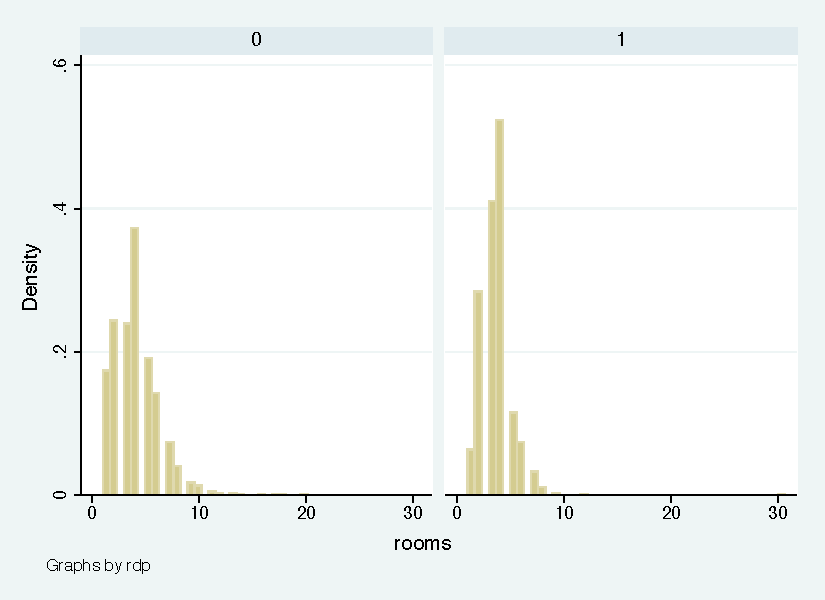
\includegraphics[scale = 0.9]{figure1.pdf}
\end{center}

\section*{Data}

The empirical analysis uses nationally representative longitudinal data that includes measures of income, employment, and housing characteristics.  The National Income Dynamics Study (NIDS) interviewed 28,000 individuals in 2008, 2010, and 2012 with a final wave for 2014 to be released this year.  In order to focus on child outcomes, I limit my analysis to children in provinces that experienced housing subsidy growth and have household incomes less than 15,000 Rand (or about 1,300 USD) per month.  The final sample includes 7,784 children of which 779 benefitted from subsidized housing over the course of the study.  I identify beneficiary status with a variable indicating whether the household received a government subsidy "to obtain this or any other dwelling."  I limit the analysis to only local housing projects where households do not report moving far to receive subsidized housing, which captures the majority of housing projects.  This approach allows me to rule out improved access to public goods or employment opportunities as part of the housing treatment.  Since I lack information on the construction date or the original owner of each house, I construct a variety of housing subsidy measures in order to exclude situations where households are joining family members in previously owned houses or benefitting from small-scale housing loan programs.  The results are robust to these alternative measures.

The summary statistics below indicate the main outcome and control variables for both residents of RDP houses and unsubsidized houses.  Looking at the raw data, I find that RDP houses are smaller yet have better services and market value.  Consistent with being a means tested program, residents of RDP houses have less income and expenditure despite many similarities in other demographic characteristics.  The main education measures of attendance and passing rates show few differences between RDP and non-RDP houses.

\begin{center}
	\input sum_1
\end {center}

\section*{Methods}

In the empirical analysis, I first explore how RDP houses and in particular the identity of the RDP homeowner affect bargaining power in the household.  I then examine the relationships between gaining access to an RDP house, the identity of the owner, and the child's school attendance.  

I construct two treatment dummy measures: "Parent Owns RDP" takes a value of one when a child's parent gains ownership of an RDP house, and "Other Family Owns RDP" takes a value of one when a non-parent family member gains ownership of an RDP house.  Both of these variables are conditional on children residing in the RDP house.  My empirical specifications take the form:

\begin{align*}
Y_{iht}  &= \beta_0 + \beta_1 ParentRDP_{iht} + \beta_2 NonParentRDP_{iht} + \gamma_t + \lambda_i + \varepsilon_{iht} \\
\end{align*}

The outcome $Y_{iht}$ varies with individual $i$, household $h$, and time $t$.  The coefficient $\beta_1$ captures the effect of a parent gaining ownership of an RDP house on the outcome while the coefficient $\beta_2$ similarly indicates the effect of a non-parent family member gaining ownership of an RDP house on the same outcome.  I include fixed effects for time and individual indicated by $\gamma_t$ and $\lambda_i$ respectively in order to account for systematic differences between individuals that might be correlated with both educational outcomes and participation in the housing program.  Since the RDP housing program is means-tested and geographically specific, it is likely that differences in outcomes between treated and untreated children cannot be entirely attributed to the housing program.  The summary statistics further indicate systematic differences between RDP and non-RDP households.  Time fixed effects similarly account for trends in outcome variables that may also correlate with treatment assignment.

In order to interpret the results as causal estimates of the impact of housing assistance, I rely on the standard differences-in-differences assumption that trends in outcome variables would be similar across treatment and control children in the absence of the housing program.  One concern is that despite the waiting-list system and quasi-random allocation of houses based on proximity to areas with low land prices, the allocation of these houses is in fact non-random due to political factors or self-selection.  If politically connected families are both more likely to benefit from their program and also invest more heavily in their children's education over time, my results may over estimate the actual impact of the program on children's education.  This bias is consistent with some allegations of corruption in the implementation of housing waiting lists.  Alternatively, households may have positive expectations of the quality of schools available to RDP houses and therefore, may petition program implementers strongly for access to a house.  This self-selection could also bias the results if these households would work to improve their children's education regardless of the housing program.

Since the substance of the results will ultimately rely on comparing treatment effects across parent and non-parent owners, I can rely on weaker assumptions to support my household bargaining theory.  I can allow for some degree of non-random selection into the program as long as this selection is symmetric across non-parent and parent owners.  For example, if parents and non-parents are equally politically-connected, then I can still interpret differences in direction or magnitude of the two treatment variables.  However, the comparison between treatment effects also requires the crucial additional assumption that the houses received by both groups are identical in quality and amenities.  For example, I would be especially concerned if program houses owned by parents are more valuable with better services than those owned by non-parent family members.  The following regression tests these assumptions by computing the mean difference between parent owned RDP houses and non-parent owned RDP houses only controlling for time and urban areas.

\begin{center}
	\input house_quality_v1
\end {center}

\pagebreak

I find that ownership of the RDP house is uncorrelated with four measures of housing quality.  This finding is consistent with the national implementation of program guidelines and reimbursement rates, effectively minimizing variation in housing quality according to demographic characteristics.  To further explore the assumption that ownership of RDP houses is uncorrelated with nearby amenities, I conduct the following series of regressions of RDP ownership on a series of school quality indicators.

\begin{center}
	\input school_quality_v1
\end {center}

I find small, insignificant coefficients for all measures of school quality except for distance in minutes to school, where I find a decline in travel time for non-parent ownership.  Given that later results associate non-parent ownership with reduced attendance, I am less concerned that access to school may improve for non-parent owned RDP houses.  While I cannot ensure that there may be unobserved differences in either house quality or school quality according to ownership of the RDP houses, these regressions help to rule out many important candidate differences.

\section*{Results}

To establish how RDP house ownership is correlated with shifts in bargaining power, I explore how RDP ownership variables affect indicators for parent as household head and grandparent as household head.  I find that parent ownership of an RDP house strongly increases the probability that a parent is the head of the household while the   The second column of the table below indicates symmetric results for grandparents.  These results suggest that shifts in the identity of the household head are strongly related to who gains ownership of the RDP house.  One explanation may be that RDP houses allow children living separately to rejoin with parents or grandparents.  The final column somewhat surprisingly shows that RDP ownership is uncorrelated with an indicator for parent coresidence, suggesting that overall household structure is not responding dramatically to the receipt of a new house.

\begin{center}
	\input first_stage_v1
\end {center}

The regressions below test for other differential demographic shifts in response to RDP home ownership.  Insignificant coefficients predicting household size and number of children children further suggest little demographic adjustment of households in response to the treatment.  The final column documents a moderate decrease in income for households where parents gain ownership of the RDP house.  This result somewhat strengthens the hypothesis of household bargaining since parents may sacrifice pooled income in forming a new household separate from grandparents.  

\begin{center}
	\input first_stage_v2
\end {center}

The main results below compute the same regressions as before except with days absent in the past month as the outcome variable.  The first column associates moving to an parent-owned RDP house with a statistically significant decline in days absent.  A larger and opposite result holds for non-parent ownership of an RDP house suggesting that shifts in bargaining power toward non-parent household members negatively impacts child education.  Column two reports results for the sample of children that report at least one day absent and matches the earlier pattern.  Column three demonstrates weaker results when the outcome variable is simply a dummy for any positive absences in the past month.  Stronger results in column two over column three suggest that changes in attendance are driven by children with already imperfect attendance (intensive margin) as opposed to children who switch from perfect to imperfect attendance (extensive margin).  Greater evidence for the intensive margin seems consistent with a theory where parents and grandparents exert influence over a child's schooling decision at this margin.  Taken together, these results suggest that shifting greater household bargaining power toward parents and away from grandparents can have very positive impacts on educational outcomes.

\begin{center}
	\input reduced_form_v1
\end {center}

The table below further supports the previous results by demonstrating increases in the probability of failing a grade for RDP houses 

%\begin{center}
%	\input reduced_form_v2
%\end {center}

\begin{center}
	\input mech_v1
\end {center}


\begin{center}
	\input robust_v1
\end {center}





\end{document}




